\documentclass[border=3pt,tikz]{standalone}
\usepackage{amsmath}
\usetikzlibrary{calc}
\usetikzlibrary{arrows.meta} % for arrow size
\begin{document}
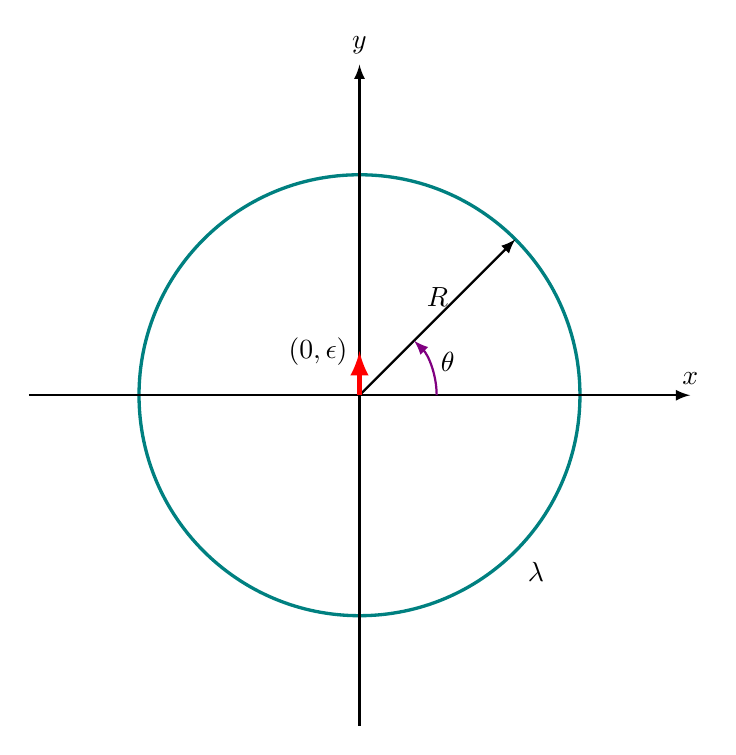
\begin{tikzpicture}[scale=1.4, rotate=0]
    \coordinate (O) at (0, 0);
    \draw[very thick, teal] (O) circle (2);
    \node at (1.6,-1.6) {$\lambda$};
    \draw[thick, -latex] (0, -3) -- (0, 3) node [above] {$y$};
    \draw[thick, -latex] (-3, 0) -- (3,0) node [above] {$x$};
    \draw[thick, -latex] (0, 0) -- node [above] {$R$} (1.414, 1.414);
    \draw[line width=0.7mm, red, -latex] (0, 0) -- (0, 0.4) node [left, black] {$(0, \epsilon)$};
    \draw[thick, violet, -latex] (0.7,0) arc (0:45:0.7);
    \node [right] at (0.65, 0.3) {$\theta$};
    \end{tikzpicture}
\end{document}